\documentclass[12pt]{extarticle} 
\usepackage{amsmath,amsfonts,amssymb,amsthm,graphicx,xcolor,natbib,enumitem,booktabs,tabularx}
%\usepackage[paperwidth=126mm, paperheight=96mm, top=5mm, bottom=5mm, right=5mm, left=5mm]{geometry}
\usepackage[margin=1cm,footskip=5mm]{geometry}
\pagenumbering{gobble}

\usepackage[BoldFont,SlantFont]{xeCJK}  
\xeCJKsetemboldenfactor{2}
\setCJKmainfont{cwTeX Q Yuan Medium}
%\setCJKmainfont{cwTeX Q Kai Medium}
%\setCJKmainfont{cwTeX Q Ming Medium}
%\setCJKmainfont[AutoFakeSlant=.1,AutoFakeBold=1]{cwTeX Q Kai Medium} 
%\setCJKfamilyfont{kaiv}[Vertical=RotatedGlyphs]{cwTeX Q Medium}
%\setmainfont{texgyrepagella-regular.otf}
%\setmathfont{texgyrepagella-math.otf}
\newcommand{\ds}{\displaystyle}
\newcommand{\ie}{\,\Longrightarrow\,}
\newcommand{\ifff}{\,\Longleftrightarrow\,}
\newcommand{\mi}{\mathrm{i}}
\DeclareMathOperator*{\dom}{dom}
\DeclareMathOperator*{\codom}{codom}
\DeclareMathOperator*{\ran}{ran}
\newcommand{\floor}[1]{\lfloor #1 \rfloor}
\newcommand{\ceil}[1]{\lceil #1 \rceil}

% figure --> 圖
\renewcommand{\appendixname}{附錄}
\renewcommand{\figurename}{圖}
\renewcommand{\tablename}{表}
\renewcommand{\refname}{參考文獻}

\usepackage{hyperref}
\hypersetup{
    colorlinks,
    linkcolor={red!50!black},
    citecolor={blue!60!black},
    urlcolor={blue!60!black}
    %urlcolor={blue!80!black}
}

\theoremstyle{definition}
\newtheorem*{dfn}{定義}
\newtheorem*{prp}{性質}
\newtheorem*{thm}{定理}
\newtheorem*{ex}{例}
\newtheorem*{rmk}{註}
\newtheorem*{sol}{解}
\newtheorem*{prf}{證}

%\setenumerate{label=(\roman*),itemsep=1pt,topsep=3pt}
\newcommand{\myline}{\noindent\makebox[\linewidth]{\rule{\paperwidth}{0.4pt}}}
%\newcommand{\myline}{\textcolor[RGB]{220,220,220}{\rule{\linewidth}{1pt}}}

\usepackage{tikz}
\usetikzlibrary{arrows.meta,angles,quotes}
\usepackage{pgfplots}
% axis style, ticks, etc
\pgfplotsset{every axis/.append style={
                   label style={font=\fontsize{4}{4}\selectfont},
                   tick label style={font=\fontsize{4}{4}\selectfont}  
               },
            }
\renewcommand\tabularxcolumn[1]{m{#1}}

\usepackage{fancyhdr}
\fancypagestyle{firststyle} {
   \fancyhf{}
   \fancyfoot[R]{\footnotesize \DTMnow}
   \renewcommand{\headrulewidth}{0pt} 
}
\usepackage{datetime2}

\usepackage{multicol}

\begin{document}
\title{\texorpdfstring{\vspace{-2em} 第零章\ \ 預備知識}{第零章\ \ 預備知識}} 
\author{\vspace{-5em}}
\date{\vspace{-5em}}
\maketitle
\thispagestyle{firststyle}

\section*{0.1 基本概念}
\subsection*{記號}

\begin{table}[!htbp]
  \centering
  \begin{tabular}{lll}
    \toprule
    $\forall$ & 對所有 & for all \\
    $\exists$ & 存在   & there exists \\
    $\exists\,!$ & 存在唯一 & there exists uniquely \\
    $\in$ & 屬於 & belongs to \\
    A $\,\Longrightarrow\,$ B &  若 A 則 B & if A then B \\
    A $\,\Longleftrightarrow\,$ B &  A 等價於 B & A if and only if B \\
    $\infty$ & 無限大 & infinity \\
    $\vee$ & 或 & or \\
    $\wedge$ & 且 & and \\
    $\because$ & 因為 & because \\
    $\therefore$ & 所以 & therefore \\
    $\neg$ & 非 & not \\
    $\equiv$ & 等價於 & is equivalent to \\
    \bottomrule
  \end{tabular}
\end{table}

\subsection*{數}

\begin{table}[!htbp]
  \centering
  \begin{tabular}{llll}
    \toprule
    $\mathbb{N}$ & 自然數 & natural number & $1,\,2,\,3,\,\ldots$ \\
    $\mathbb{Z}$ & 整數   & integer & $\ldots,\,-2,\,-1,\,0,\,1,\,2,\,\ldots$\\
    $\mathbb{Q}$ & 有理數 & rational number & $\ds\frac{p}{q}: \,p,\,q\in\mathbb{Z}$ \\
    $\mathbb{R}$ & 實數 & real number &  \\
    $\mathbb{C}$ & 複數 & complex number & $\ds\alpha + \beta\,\mi: \,\alpha,\,\beta\in\mathbb{R},\,\mi = \sqrt{-1}$ \\
    \bottomrule
  \end{tabular}
\end{table}

\subsection*{集合}

\begin{table}[!htbp]
  \centering
  \begin{tabular}{lll}
    \toprule
    $x\in S$ & $x$ 為集合 $S$ 的元素 &  \\
    $S_1 =\{x_1, x_2, \ldots\}$ & 列舉式   &  \\
    $S_2 =\{ x\,|\, x \text{ 滿足某性質}\}$ & 敘述式 & \\
    $S\cap T$ & $\{x\,|\, x\in S\,\wedge\,x\in T\}$ & 交集 (intersection)    \\
    $S\cup T$ & $\{x\,|\, x\in S\,\vee\,x\in T\}$ & 聯集 (union)    \\
    $S\setminus T$ & $\{x\,|\, x\in S\,\wedge\,x\not\in T\}$ & 差集 (difference)   \\
    $S\times T$ & $\{(x, y)\,|\, x\in S\,\wedge\,y\in T\}$ & 積集 (Cartesian product)  \\
    $\varnothing$ & 空集合 & \\
    $S_1\subset S_2$, $S_2\supset S_1$ & $S_1$ 為 $S_2$ 的真子集合 & \\
    $S_1\subseteq S_2$, $S_2\supseteq S_1$ & $S_1$ 為 $S_2$ 的子集合 & \\
    $\ds\cap_{i=1}^n S_i$ & $S_1\cap S_2\cap\cdots\cap S_n$ &    \\
    $\ds\cup_{i=1}^n S_i$ & $S_1\cup S_2\cup\cdots\cup S_n$ &    \\
    \bottomrule
  \end{tabular}
\end{table}

\newpage

\subsection*{區間}

\begin{table}[!htbp]
  \centering
  \begin{tabular}{lll}
    \toprule
    $(a, b) = \{x\,|\,a < x < b\}$ & 端點為 $a$, $b$ 的開區間 &  \\%open interval with endpoints $a$, $b$\\
    $[a, b] = \{x\,|\,a \leqslant x \leqslant b\}$ & 端點為 $a$, $b$ 的閉區間 & \\%closed interval with end points $a$, $b$\\
    $[a, b) = \{x\,|\,a \leqslant x < b\}$ & \\%端點為 $a$, $b$ 的半開區間 &  \\
    $(a, b] = \{x\,|\,a < x \leqslant b\}$ & \\%端點為 $a$, $b$ 的半開區間 &  \\
    $(a, \infty) = \{x\,|\,a < x\}$ & \\%端點為 $a$ 的無窮區間 &  infinite interval with left endpoint $a$\\
    $[a, \infty) = \{x\,|\,a \leqslant x\}$ & \\%端點為 $a$ 的無窮區間 &  infinite interval with left endpoint $a$ included\\
    $(-\infty, b) = \{x\,|\, x < b\}$ & \\%端點為 $b$ 的無窮區間 & infinite interval with right endpoint $b$ \\
    $(-\infty, b] = \{x\,|\, x \leqslant b\}$ & \\%端點為 $b$ 的無窮區間 &  infinite interval with right endpoint $b$ included\\
    \bottomrule
  \end{tabular}
\end{table}

\subsection*{不等式}
\begin{prp}
  令 $a, b, c\in\mathbb{R}$. 
  \setlength{\columnsep}{-20mm}
  \begin{multicols}{2}
    \begin{enumerate}\setlength\itemsep{0em}
      \item $\ds a < b \ie a + c < b + c$
      \item $\ds a < b, \,c < d \ie a + c < b + d$
      \item $\ds a < b, \,c > 0 \ie a c < b c$
      \item $\ds a < b, \,c < 0 \ie a c > b c$
      \item $\ds0 < a < b \ie \frac{1}{a} > \frac{1}{b}$
    \end{enumerate}
  \end{multicols}
\end{prp}

\begin{ex}
  解下列不等式. 
  \setlength{\columnsep}{-20mm}
  \begin{multicols}{2}
    \begin{enumerate}\setlength\itemsep{0em}
      \item $\ds 2x - 3 < x + 4 < 3 x - 2$
      \item $\ds x^3 > x$
      \item $\ds (2 - x)(1 - x)^2 x^3 \leqslant 0$
      \item $\ds -2 < \frac{2x - 3}{x + 1} < 1$
    \end{enumerate}
  \end{multicols}
\end{ex}

\begin{sol}
  \begin{enumerate}\setlength\itemsep{0em}
    \item[]
    \item $\ds 3 < x < 7$
    \item $\ds x^3 - x > 0 \ie x(x^2 - 1) > 0 \ie x(x + 1)(x - 1) > 0 \ie x > 1 \vee -1 < x < 0$
    \item $\ds (2 - x)(1 - x)^2 x^3 \leqslant 0 \ie (x - 2)(x - 1)^2 x^3 \geqslant 0 \ie x\geqslant 2 \vee x\leqslant 0\vee x = 1$
    \item $\ds -2 < \frac{2x - 3}{x + 1} < 1 \ie \Big(-2 < \frac{2x - 3}{x + 1}\Big)\wedge\Big(\frac {2x - 3}{x + 1} < 1\Big) \ie \Big(\frac{4x - 1}{x + 1} > 0\Big) \wedge \Big(\frac{x - 4}{x + 1} < 0\Big) \\ \ie \Big(x < -1 \vee x > \frac{1}{4}\Big) \wedge (-1 < x < 4) \ie \frac{1}{4} < x < 4$
  \end{enumerate}
\end{sol}

\myline

\subsection*{絕對值}
令 $a\in\mathbb{R}$;  $a$ 的絕對值 (absolute value) $|a|$ 定義為 $\ds|a|=\begin{cases} a & \text{若}\;a\geqslant 0 \\ - a&\text{若}\;a < 0\end{cases}$

\begin{prp}
  若 $a > 0$, 則
  \setlength{\columnsep}{-20mm}
  \begin{multicols}{3}
    \begin{enumerate}\setlength\itemsep{0em}
      \item $\ds |x| = a \ifff x = \pm\,a$
      \item $\ds |x| < a \ifff -a < x < a$
      \item $\ds |x| > a \ifff x < -a \,\vee\, x > a$
    \end{enumerate}
  \end{multicols}
\end{prp}

\begin{prp}
  若 $a, b\in\mathbb{R}$, 則
  \setlength{\columnsep}{-20mm}
  \begin{multicols}{3}
    \begin{enumerate}\setlength\itemsep{0em}
      \item $\ds |-a| = |a|$
      \item $\ds \sqrt{a^2} = |a|$
      \item $\ds |a b| = |a|\,|b|$
      \item $\ds \Big|\frac{b}{a}\Big| = \frac{|b|}{|a|}$
      \item $\ds |a + b|\leqslant|a| + |b|$
      \item $\ds \big|\,|a| - |b|\,\big|\leqslant|a - b|$
    \end{enumerate}
  \end{multicols}
\end{prp}

\begin{prf}[不等式]
  \begin{itemize}\setlength\itemsep{0em}
    \item[]
    \item $\ds (|a + b|)^2 = (a + b)^2 = a^2 + 2 a b + b^2 = |a|^2 + 2 a b + |b|^2 \leqslant |a|^2 + 2 |a b| + |b|^2 = |a|^2 + 2 |a|\,|b| + |b|^2 = (|a| + |b|)^2$, 故 $\ds |a + b|\leqslant|a| + |b|$. 
    \item $\ds |a| = |(a - b) + b| \leqslant |a - b| + |b| \ie |a| - |b| \leqslant |a - b|$;  $\ds |b| = |(b - a) + a| \leqslant |b - a| + |a| = |a - b| + |a| \ie |a| - |b| \geqslant -|a - b|$.  故 $\ds \big|\,|a| - |b|\,\big|\leqslant|a - b|$. 
  \end{itemize}
\end{prf}

\begin{ex}
  解下列不等式與方程式. 
  \setlength{\columnsep}{-20mm}
  \begin{multicols}{3}
    \begin{enumerate}\setlength\itemsep{0em}
      \item $\ds |5 - 2x| < 3$
      \item $\ds \Big|\frac{2 x - 1}{x + 1}\Big| = 3$
      \item $\ds |x - 1| - |x - 10|\geqslant 5$
    \end{enumerate}
  \end{multicols}
\end{ex}

\begin{sol}
  \begin{enumerate}\setlength\itemsep{0em}
    \item[]
    \item $\ds |5 - 2x| < 3 \ie -3 < 5 - 2x < 3 \ie -8 < -2x < -2 \ie 1 < x < 4$
    \item $\ds \Big|\,\frac{2 x - 1}{x + 1}\,\Big| = 3 \ie \frac{2 x - 1}{x + 1} = 3\,\vee\,\frac{2 x - 1}{x + 1} = -3 \ie x = -4 \,\vee\, x = -\frac{2}{5}$
    \item 當 $x < 1$, $\ds |x - 1| - |x - 10|\geqslant 5 \ie (1 - x) - (10 - x)\geqslant 5 \ie -9 \geqslant 5$, 不合. 當 $1\leqslant x < 10$, $\ds |x - 1| - |x - 10|\geqslant 5 \ie (x - 1) - (10 - x)\geqslant 5 \ie 2 x\geqslant 16 \ie x\geqslant 8$, 則 $8\leqslant x < 10$. 當 $x\geqslant 10$, $\ds |x - 1| - |x - 10|\geqslant 5 \ie (x - 1) - (x - 10)\geqslant 5 \ie 9\geqslant 5$ 恆成立. 綜上, $8\leqslant x$. 
  \end{enumerate}
\end{sol}

\subsection*{平面幾何}

\begin{prp}
  \begin{itemize}\setlength\itemsep{0em}
    \item[]
    \item $P_1: (x_1, y_1)$ 與 $P_2: (x_2, y_2)$ 之距離為 $\ds \sqrt{(x_1 - x_2)^2 + (y_1 - y_2)^2}$
    \item 一非鉛直線通過 $P_1: (x_1, y_1)$ 與 $P_2: (x_2, y_2)$, 則直線斜率 $m$ 為 $\ds m = \frac{\Delta y}{\Delta x} = \frac{y_2 - y_1}{x_2 - x_1}$
    \item 直線方程式表示法 --- 點斜式: $\ds y - y_1 = m(x - x_1)$; $\;$ 斜截式: $\ds y = m x + b$; $\;$ 截距式: $\ds \frac{x}{a} + \frac{y}{b} = 1$
    \item 兩非鉛直線 --- 平行:  斜率相等; 垂直:  斜率相乘為 $-1$
  \end{itemize}
\end{prp}

\section*{0.2 函數}

\begin{dfn}
  \begin{itemize}\setlength\itemsep{0em}
    \item[]
    \item 函數 (function) $f:A\to B$ 是一個對應關係: 對所有 $a\in A$, 存在唯一 $b\in B$, 使得 $f$ 將 $a$ 對應到 $b$. $\ds\forall\,a\in A\;\exists\,!\,b\in B\;(f(a) = b)$.
    \item $A$ --- 定義域 (domain): $\dom f = A$; $\quad B$ --- 對應域 (codomain): $\codom f = B$ \\
          $f(A) = \{f(a)\,|\,a\in A\}\subseteq B$ --- 值域 (range): $\ran f \equiv f(A)$      
  \end{itemize}
\end{dfn}

\begin{rmk}[函數形式]
  \begin{itemize}\setlength\itemsep{0em}
    \item[]
    \item 公式型 --- $y = f(x) = 3x + 1$, $\dom f = \ran f = \mathbb{R}$; $y = f(x) = 3x^2 + 1$, $\dom f = \mathbb{R}$, $\ran f = \{x\,|\, x\geqslant 1\}$; $y = f(x) = \sin\pi x$, $\dom f = \mathbb{R}$, $\ran f = [-1, 1]$.
    \item 抽象型 --- 例: 令 $A = \{\text{Mon},\,\text{Tue},\,\text{Wed},\,\text{Thu},\,\text{Fri}\}$, $B = \{\text{a},\,\text{b},\,\text{c}, \ldots,\,\text{z}\}$, 定義函數 $f:A\to B$ 使得 \\$f(\text{工作日}) = (\text{開頭小寫英文字母})$: $f(\text{Mon}) = \text{m}$, $f(\text{Wed}) = \text{w}$, $f(\text{Tue}) = f(\text{Thu}) = \text{t}$, $f(\text{Fri}) = \text{f}$. 故 $\dom f = A$, $\codom f = B$, $\ran f = \{\text{m},\,\text{w},\,\text{t},\,\text{f}\}$. 
  \end{itemize}
\end{rmk}

\begin{ex}
  $f(x) = \sqrt{-x^2 + x + 2}$, 求 $\dom f$ 與 $\ran f$. 
\end{ex}

\begin{sol}
  由 $-x^2 + x + 2 = -(x + 1)(x - 2)\geqslant 0 \ie (x + 1)(x - 2)\leqslant 0 \ie -1\leqslant x\leqslant 2$, $\dom f = [-1, 2]$. 又 $-x^2 + x + 2 = -\big(x - \frac{1}{2}\big)^2 + \frac{9}{4}$, 當 $x\in [-1, 2]$ 時, $f(x)\in\big[0, \sqrt{\frac{9}{4}}\big] = \big[0, \frac{3}{2}\big]$, 故 $\ran f = \big[0, \frac{3}{2}\big]$. 
\end{sol}

\begin{ex}
  $\ds f(x) = \frac{1}{(x-2)(x-3)}$, 求 $\dom f$ 與 $\ran f$. 
\end{ex}

\begin{sol}
  $\dom f = \mathbb{R}\setminus\{2, 3\}$. 令 $\ds y = \frac{1}{(x - 2)(x - 3)} = \frac{1}{x^2 - 5x + 6}\ie x^2 - 5 x + \big(6 - \frac{1}{y}\big) = 0$. 當判別式 $\geqslant 0$ 時有實數解 $\ds\ie (-5)^2 - 4\,\Big(6 - \frac{1}{y}\Big)\geqslant 0 \ie 1 + \frac{4}{y}\geqslant 0 \ie \frac{y + 4}{y}\geqslant 0$, 故 $\ds\ran f = \{y\,|\,y > 0\,\vee\,y\leqslant -4\}$. 
\end{sol}

\subsection*{嵌射與蓋射}
\begin{dfn} 給定函數 $f: A\to B$. 
  \begin{itemize}\setlength\itemsep{0em}
    \item $f$ 為嵌射 (one-to-one, injective): $\forall\,x_1, x_2\in A\;(f(x_1) = f(x_2) \ie x_1 = x_2)$. 
    \item $f$ 為蓋射 (onto, surjective): $\forall\,b\in B\;\exists\,a\in A\;(f(a) = b)$. 
  \end{itemize}
\end{dfn}

\myline

%\begin{rmk}[邏輯推理原則]
%  \begin{itemize}\setlength\itemsep{0em}
%    \item[]
%    \item 令 $p$, $q$ 為兩邏輯敘述: $(p \ie q) \,\equiv\, (\neg\,q \ie \neg\,p)$
%    \item ``若下雨, 則帶傘'' $\equiv$ ``若沒帶傘, 則沒下雨''
%    \item ``若下雨, 則帶傘'' $\not\equiv$ ``若沒下雨, 則沒帶傘''
%    \item ``若 $x = 2$, 則 $x$ 為偶數'' $\equiv$ ``若 $x$ 不為偶數, 則 $x\ne 2$''
%    \item ``若 $x = 2$, 則 $x$ 為偶數'' $\not\equiv$ ``若 $x\ne 2$, 則 $x$ 不為偶數'' !
%    \item $\ds \left(\left(f(x_1) = f(x_2)\right) \ie \left(x_1 = x_2\right)\right) \,\equiv\, \left(\left(x_1 \ne x_2\right) \ie \left(f(x_1) \ne f(x_2)\right)\right)$. 
%  \end{itemize}
%\end{rmk}

\begin{ex}
  證明函數 $f:\mathbb{R}\to\mathbb{R}$, $f(x) = 2x + 1$ 為嵌射. 
\end{ex}

\begin{sol}
  $\forall\,x_1, x_2\in\mathbb{R}$, $f(x_1) = f(x_2) \ie (2 x_1 + 1) = (2 x_2 + 1) \ie x_1 = x_2$.  
\end{sol}

\begin{ex}
  \begin{itemize}\setlength\itemsep{0em}
    \item[]
    \item 說明函數 $f:\mathbb{R}\to\mathbb{R}$, $f(x) = x^2$ 不為嵌射. 
    \item 證明函數 $f:\mathbb{R}_+= \{x\,|\,x\geqslant 0\}\to\mathbb{R}$, $f(x) = x^2$ 為嵌射.
  \end{itemize}
\end{ex}

\begin{sol}
  \begin{itemize}\setlength\itemsep{0em}
    \item[]
    \item 取 $x_1 = 1$, $x_2 = -1$, $x_1\ne x_2$, 但 $f(x_1) = f(x_2) = 1$.  
    \item $\forall\,x_1, x_2\in\mathbb{R}$, $\ds f(x_1) = f(x_2) \ie x_1^2 = x_2^2 \ie (x_1 - x_2)(x_1 + x_2) = 0 \ie x_1 - x_2 = 0 \,\vee\, x_1 + x_2 = 0 \ie x_1 = x_2 \,\vee\, x_1 = x_2 = 0\ie x_1 = x_2$.  
  \end{itemize}
\end{sol}

\begin{ex}
  證明函數 $f:\mathbb{R}\to\mathbb{R}$, $f(x) = x^3$ 為嵌射. 
\end{ex}

\begin{sol}
  $\forall\,x_1, x_2\in\mathbb{R}$, $\ds f(x_1) = f(x_2) \ie x_1^3 = x_2^3 \ie (x_1 - x_2)(x_1^2 + x_1 x_2 + x_2^2) = 0 \ie x_1 - x_2 = 0\,\vee\, x_1^2 + x_1 x_2 + x_2^2 = 0 \ie x_1 = x_2\,\vee\,\Big(x_1 + \frac{x_2}{2}\Big)^2 + \frac{3x_2^2}{4} = 0 \ie x_1 = x_2\,\vee\, \Big(x_2 = 0 \,\wedge\, x_1 + \frac{x_2}{2} = 0\Big) \ie x_1 = x_2\,\vee\, x_2 = x_1 = 0 \ie x_1 = x_2$.  
\end{sol}

%\begin{ex}
%  令 $\mathbb{Z}^+ = \mathbb{N}\cup\{0\}$. 定義函數 $f:\mathbb{Z}^+\times\mathbb{Z}^+\to\mathbb{Z}^+$ 為 $\ds f(m, n) = \frac{(m + n)(m + n + 1)}{2} + m$. 證明 $f$ 為嵌射, 亦為蓋射. 
%\end{ex}
%
%\begin{sol}
%  \begin{itemize}\setlength\itemsep{0em}
%    \item[]
%    \item (嵌射) 設 $f(m_1, n_1) = f(m_2, n_2)$. 令 $k_1 = m_1 + n_1$, $k_2 = m_2 + n_2$, 則 $\ds f(m_1, n_1) = \frac{k_1(k_1 + 1)}{2} + m_1$,  $\ds f(m_2, n_2) = \frac{k_2(k_2 + 1)}{2} + m_2$. 由 $f(m_1, n_1) = f(m_2, n_2) \ie k_1(k_1 + 1) + 2 m_1 = k_2(k_2 + 1) + 2 m_2 \ie k_1^2 + k_1 - k_2^2 - k_2 = 2(m_2 - m_1) \ie (k_1 - k_2)(k_1 + k_2 + 1) = 2(m_2 - m_1)$. 若 $k_1 = k_2$, 則 $m_2 = m_1$, 亦即 $n_2 = n_1$. 若 $k_1\not=k_2$, WLOG $k_1 > k_2$, 則 $2(m_2 - m_1) = (k_1 - k_2)(k_1 + k_2 + 1)\geqslant k_1 + k_2 + 1 > 2k_2 + 1\geqslant 2m_2 + 2n_2 + 1 > 2m_2$, 矛盾. 
%    \item (蓋射) 給定任意 $l\in\mathbb{N}$. 由於整數列 $\ds\frac{k(k + 1)}{2}$ 遞增且 $\ds\frac{(k+1)(k+2)}{2} - \frac{k(k + 1)}{2} = k + 1$, 存在 $k\in\mathbb{N}$ 使 $\ds\frac{k(k+1)}{2}\leqslant l < \frac{(k + 1)(k + 2)}{2}$. 令 $\ds m = l - \frac{k(k + 1)}{2}$, $\ds n = k - m = k + \frac{k(k + 1)}{2} - l = \frac{(k + 1)(k + 2)}{2} - 1 - l\geqslant 0$, 則 $m, n\in\mathbb{Z}^+$ 且 $f(m, n) = l$.   
%  \end{itemize}
%\end{sol}

\section*{0.3 函數運算}

\begin{table}[!htbp]
  \centering
  \begin{tabular}{lll}
    \toprule
    $\ds (f\pm g)(x) = f(x)\pm g(x)$ & $\dom(f\pm g) = \dom f\,\cap\,\dom g$ &  \\
    $\ds (f\cdot g)(x) = f(x)\cdot g(x)$ & $\dom(f\cdot g) = \dom f\,\cap\,\dom g$ &  \\
    $\ds \Big(\frac{f}{g}\Big)(x) = \frac{f(x)}{g(x)}$ & $\ds\dom\frac{f}{g} = \dom f\,\cap\,\dom g\,\setminus\,\{ x\,|\,g(x) = 0\}$ &  \\
    $\ds (f\circ g)(x) = f(g(x))$ & $\dom(f\circ g) = \{ x\in\dom g\,|\,g(x)\in\dom f\}$ &  \\
    \bottomrule
  \end{tabular}
\end{table}

\begin{ex}
  \begin{enumerate}\setlength\itemsep{0em}
    \item[]
    \item 設 $\ds f\Big(x - \frac{1}{x}\Big) = x^2 + \frac{1}{x^2}$, 求 $f(2)$. 
    \item 設 $f(x) = x$, $\ds g(x) = \frac{1}{x}$, $\ds h(x) = (f\cdot g)(x) = x\cdot\frac{1}{x} = 1$, 求 $\dom h$. 
    \item 設 $F(x) = \sin^3(x + 3)$, 求函數 $f$, $g$, $h$ 使得 $F = f\circ g\circ h$. 
    \item 設 $\ds f(x) = \frac{x + 1}{1 + \frac{1}{x + 1}}$, 求 $\dom f$. 
    \item 設 $\ds f(x) = \sqrt{x}$, $g(x) = \sqrt{2 - x}$, 求 $f\circ f$, $f\circ g$, $g\circ f$, $g\circ g$, 以及其定義域. 
    \item 設 $\ds g(x) = 2x + 1$, $h(x) = 4x^2 + 4x + 7$.
      \setlength{\columnsep}{-0mm}
      \begin{multicols}{2}
        \begin{itemize}\setlength\itemsep{0em}
          \item 求函數 $f(x)$ 使得 $f\circ g = h$. 
          \item 求函數 $f(x)$ 使得 $g\circ f = h$. 
        \end{itemize}
      \end{multicols}
    \item 若 $\ds f_0(x) = \frac{x}{x + 1}$, $\ds f_{n+1} = f_0\circ f_n$, $n = 0,\,1,\,2,\,\ldots$. 求 $f_n(x)$ 之公式.  
  \end{enumerate}
\end{ex}

% There's no such function $f$ s.t. $f(f(z)) = az^2 + bz + c$: See: Rice R. E., Schweizer B., Sklar A. When is $f(f(z)) = az^2 + bz + c$, The American Mathematical Monthly, Vol. 87, No. 4. (Apr., 1980), pp. 252-263, \href{http://yaroslavvb.com/papers/rice-when.pdf}{link}

\begin{sol}
  \begin{enumerate}\setlength\itemsep{0em}
    \item[] 
    \item 若 $\ds x - \frac{1}{x} = 2$, $\ds 4 = \Big(x - \frac{1}{x}\Big)^2 = x^2 - 2 + \frac{1}{x^2}\ie x^2 + \frac{1}{x^2} = 6$. 由 $\ds f\Big(x - \frac{1}{x}\Big) = x^2 + \frac{1}{x^2}$, $f(2) = 6$. 
    \item 由 $\dom(f\cdot g) = \dom f\,\cap\,\dom g$, $\dom h = \mathbb{R}\,\cap\,\big(\mathbb{R}\setminus\{0\}\big) = \mathbb{R}\setminus\{0\}$. 
    \item $f(x) = x^3$, $g(x) = \sin x$, $h(x) = x + 3$. 
    \item 由 $\ds\dom\frac{f}{g} = \dom f\,\cap\,\dom g\,\setminus\,\{ x\,|\,g(x) = 0\}$, $\dom f = \mathbb{R}\,\cap\,\big(\mathbb{R}\cap\big(\mathbb{R}\setminus\{-1\}\big)\big)\setminus\big\{x\,|\,1 + \frac{1}{x + 1} = 0\big\} \\= \mathbb{R}\setminus\{-1, -2\}$
    \item $f\circ f = \sqrt[4]{x}$, $f\circ g = \sqrt[4]{2 - x}$, $g\circ f = \sqrt{2 - \sqrt{x}}$, $g\circ g = \sqrt{2 - \sqrt{2 - x}}$, $\dom f\circ f = [0, \infty)$, $\dom f\circ g = (-\infty, 2]$, $\dom g\circ f = [0, 4]$, $\dom g\circ g = [-2, 2]$. 
    \item $f(x) = x^2 + 6$, $f(x) = 2x^2 + 2x + 3$. 
    \item 使用數學歸納法驗證 $\ds f_n(x) = \frac{x}{(n + 1)\,x + 1}$. 
  \end{enumerate}
\end{sol}

\section*{0.4 函數圖形}

\begin{dfn}
  若 $A$, $B\subseteq\mathbb{R}$, 則函數 $f: A\to B$ 稱為實數值函數 (real-valued function) , 集合 $\{(x, f(x))\,|\,x\in A\}$ 稱為 $f$ 的圖形 (graph) . 
\end{dfn}

\begin{prp}函數 / 圖形判斷法
  \begin{itemize}\setlength\itemsep{0em}
    \item 垂直線判斷法: 函數圖形 $\ifff$ 任一垂直線與其至多交於一點
    \item 水平線判斷法: 嵌射圖形 $\ifff$ 任一水平線與其至多交於一點
  \end{itemize}
\end{prp}

\begin{prp}變換後圖形方程式
  \setlength{\columnsep}{-0mm}
  \begin{multicols}{2}
  \begin{itemize}\setlength\itemsep{0em}
    \item 垂直平移:  $y = f(x) + h$
    \item 水平平移:  $y = f(x + h)$
    \item 垂直伸縮:  $y = c\,f(x)$
    \item 水平伸縮:  $y = f(c\,x)$
    \item $y = -f(x)$ 為 $y = f(x)$ 對 $x$ 軸的鏡射. 
    \item $y = f(-x)$ 為 $y = f(x)$ 對 $y$ 軸的鏡射. 
  \end{itemize}
\end{multicols}
\end{prp}

\section*{0.5 函數範例}

\begin{ex}分段定義函數
  \begin{itemize}\setlength\itemsep{0em}
    \item $\ds|x| = \begin{cases} x & x\geqslant 0 \\ -x & x< 0\end{cases}$
    \item  (最大整數 / Gauss / 地板) 函數 (greatest integer / Gauss / floor) $\floor{x}$ \\
      $\ds\floor{x} = n$, 若 $n\leqslant x < n + 1$, $n\in\mathbb{Z}$. $\floor{x}$ 為小於或等於 $x$ 的最大整數.     
    \item 天花板函數 (ceiling) $\ceil{x}$ \\
      $\ds\ceil{x} = n + 1$, 若 $n < x \leqslant n + 1$, $n\in\mathbb{Z}$. $\ceil{x}$ 為大於或等於 $x$ 的最小整數. 
    \item $\ds\ceil{x} = -\floor{-x}$. 
    \item 若 $g$, $h$ 為實數值函數, 則 $\ds f(x) = \max\,\{g(x),\,h(x)\} = \frac{|g(x) - h(x)|}{2} + \frac{g(x) + h(x)}{2}$. 
  \end{itemize}
\end{ex}

\myline

\section*{0.6 函數特性}
\subsection*{奇偶性}
\begin{dfn} 給定實數值函數 $f$, $\forall x\in\dom f$ 
  \begin{itemize}\setlength\itemsep{0em}
    \item 若 $f(-x) = f(x)$, 則 $f$ 為偶函數 (even function) . 
    \item 若 $f(-x) = -f(x)$, 則 $f$ 為奇函數 (odd function) . 
  \end{itemize}
\end{dfn}

\begin{prp}
  任意實數值函數可唯一表示成一個偶函數與一個奇函數的和. 
\end{prp}

\begin{prf} 設實數值函數為 $f$. 
  \begin{itemize}\setlength\itemsep{0em}
    \item (存在性) 令 $\ds E(x) = \frac{f(x) + f(-x)}{2}$, $\ds O(x) = \frac{f(x) - f(-x)}{2}$, 則 $E$ 為偶函數, $O$ 為奇函數, $f(x) = E(x) + O(x)$. 
    \item (唯一性) 已知 $\ds f(x) = E_1(x) + O_1(x) = E_2(x) + O_2(x)$. 令 $E_1(x) - E_2(x) = e(x)$, $O_1(x) - O_2(x) = o(x)$, 則 $e(x)$ 為偶函數, $o(x)$ 為奇函數, 且 $e(x) + o(x) = 0$. 若 $x\leftarrow -x$, 則 $e(-x) + o(-x) = 0 \ie e(x) - o(x) = 0$, 故 $e(x) = 0$, $o(x) = 0$. 
  \end{itemize}
\end{prf}

\subsection*{增減性}

\begin{dfn} 給定實數值函數 $f$ 與區間 $I$. $\forall\,x, y\in I$, $x < y$: 
  \begin{itemize}\setlength\itemsep{0em}
    \item 若 $f(x) < f(y)$, 則稱 $f$ 在 $I$ 為嚴格遞增 / 嚴格上升 (increasing) . 
    \item 若 $f(x) > f(y)$, 則稱 $f$ 在 $I$ 為嚴格遞減 / 嚴格下降 (decreasing) . 
    \item 若 $f(x) \leqslant f(y)$, 則稱 $f$ 在 $I$ 為遞增 / 上升 (non-decreasing) . 
    \item 若 $f(x) \geqslant f(y)$, 則稱 $f$ 在 $I$ 為遞減 / 下降 (non-increasing) . 
  \end{itemize}
\end{dfn}

\section*{0.7 反函數}

\begin{dfn}
  若函數 $f$ 為嵌射, 則其反函數 $f^{-1}:\ran f\to\dom f$ 定義為 $f^{-1}(b) = a \ifff f(a) = b$, 其中 $a\in\dom f$, $b\in\ran f$. 
\end{dfn}

\begin{prp}[常用規則] 
  \setlength{\columnsep}{-0mm}
  \begin{multicols}{2}
    \begin{enumerate}\setlength\itemsep{0em}
      \item $f^{-1}(y) = x \ifff f(x) = y$
      \item $\dom f^{-1} = \ran f$, $\ran f^{-1} = \dom f$
      \item $\ds f^{-1}(x) = (f(x))^{-1} \ne \frac{1}{f(x)} $
      \item $(f^{-1}\circ f)(x) = x$, $\forall\,x\in\dom f$
      \item $(f\circ f^{-1})(y) = y$, $\forall\,y\in\dom f^{-1} = \ran f$
      \item $y = f(x)$ 與 $y = f^{-1}(x)$ 之圖形對 $y = x$ 對稱. 
      \item 若 $f$ 為嚴格遞增或嚴格遞減函數, 則 $f$ 為嵌射 $\ie$ 存在 $f^{-1}$. 
    \end{enumerate}
  \end{multicols}
\end{prp}

\begin{ex}
  令 $f(x) = \sin x$, 若定義在
  \setlength{\columnsep}{-6cm}
  \begin{multicols}{2}
    \begin{itemize}\setlength\itemsep{0em}
      \item $[0, \pi]$ 時, 非為嵌射 (一對一) 
      \item $\big[\frac{-\pi}{2}, \frac{\pi}{2}\big]$ 時為嚴格遞增, 存在反函數 $\sin^{-1}:[-1, 1]\to\big[\frac{-\pi}{2}, \frac{\pi}{2}\big]$
    \end{itemize}
  \end{multicols}
\end{ex}

\begin{ex} 
  %\setlength{\columnsep}{-0mm}
  %\begin{multicols}{2}
    \begin{enumerate}\setlength\itemsep{0em}
      \item[]
      \item 求 $f(x) = x^3 + 2$ 的反函數. 
      \item 求 $f(x) = x^2$, $x\geqslant 0$ 的反函數, 並求 $x\leqslant 0$ 時的反函數.
      \item 求 $\ds f(x) = \frac{1 + 9 x}{4 - x}$, $x < 4$ 的反函數. 
    \end{enumerate}
  %\end{multicols}
\end{ex}

\begin{sol} 
  \begin{enumerate}\setlength\itemsep{0em}
    \item[]
    \item $y = x^3 + 2$; $x\longleftrightarrow y$: $x = y^3 + 2 \ie y^3 = x - 2 \ie y = \sqrt[3]{x - 2} \ie f^{-1}(x) = \sqrt[3]{x - 2}$.  
    \item $y = x^2$, $x\geqslant 0$;  $x\longleftrightarrow y$: $x = y^2 \ie y^2 = x \ie y = \sqrt{x} \ie f^{-1}(x) = \sqrt{x}$; $f^{-1}:[0, \infty)\to [0, \infty)$. \\$y = x^2$, $x\leqslant 0$;  $x\longleftrightarrow y$: $x = y^2 \ie y^2 = x \ie y = -\sqrt{x} \ie f^{-1}(x) = -\sqrt{x}$; $f^{-1}:[0, \infty)\to (-\infty, 0]$. 
    \item $\ds f(x) = \frac{1 + 9x}{4 - x} \ie y = \frac{1 + 9x}{4 - x}$; $x\longleftrightarrow y$: $\ds x = \frac{1 + 9 y}{4 - y} \ie y = \frac{4 x - 1}{x + 9} \ie f^{-1}(x) = \frac{4 x - 1}{x + 9}$. \\
      檢驗: $\ds (f^{-1}\circ f)(x) = f^{-1}(f(x)) = \frac{4\cdot\frac{1 + 9x}{4 - x} - 1}{\frac{1 + 9x}{4 - x} + 9} = \frac{\frac{4 + 36 x - 4 + x}{4 - x}}{\frac{1 + 9x + 36 - 9x}{4 - x}} = \frac{37 x}{37} = x$; $\ds(f\circ f^{-1})(x) = f(f^{-1}(x)) = \frac{1 + 9\cdot\frac{4x - 1}{x + 9}}{4 - \frac{4 x - 1}{x + 9}} = \frac{\frac{x + 9 + 36 x - 9}{x + 9}}{\frac{4 x + 36 - 4x + 1}{x + 9}} = \frac{37x}{37} = x$. 
  \end{enumerate}
\end{sol}

\section*{0.8 指數函數}

$y = f(x) = a^x$, $a > 0\,\wedge\, a\not=1$. 

\begin{figure}[!htbp]
  \centering
  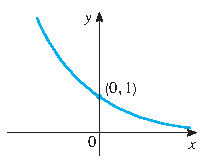
\includegraphics[width=.3\textwidth,page=1]{fig/power.pdf}\hspace{2cm}
  \includegraphics[width=.3\textwidth,page=2]{fig/power.pdf}
  \caption{$y = a^x$: 圖左 $0 < a < 1$, 圖右 $a > 1$}
\end{figure}

\vspace{-5mm}
\begin{prp} 若 $a$, $b > 0$, $x$, $y\in\mathbb{R}$, 則
  \setlength{\columnsep}{-0mm}
  \begin{multicols}{3}
    \begin{itemize}\setlength\itemsep{0em}
      \item $\ds a^x\cdot a^y = a^{x + y}$
      \item $\ds a^{-x} = \frac{1}{a^x}$
      \item $\ds\frac{a^x}{a^y} = a^{x - y}$
      \item $\ds (a^x)^y = a^{xy} = (a^y)^x$
      \item $\ds a^x\cdot b^x = (ab)^x$
      \item $\ds\frac{a^x}{b^x} = \Big(\frac{a}{b}\Big)^x$
    \end{itemize}
  \end{multicols}
\end{prp}

\myline

\section*{0.9 對數函數}

$y = f(x) = \log_a x$, $a > 0\,\wedge a\not=1$. 

\begin{figure}[!htbp]
  \centering
  \includegraphics[width=.3\textwidth,page=3]{fig/power.pdf}\hspace{2cm}
  \includegraphics[width=.3\textwidth,page=4]{fig/power.pdf}
  \caption{$y = \log_a x$}
\end{figure}

\begin{prp} 給定 $a > 0\,\wedge a\not=1$, $x > 0$, $y\in\mathbb{R}$. 
  \setlength{\columnsep}{-0mm}
  \begin{multicols}{3}
    \begin{itemize}\setlength\itemsep{0em}
      \item $\log_a x = y \ifff a^y = x$
      \item $\ds\log_a a^y = y$
      \item $\ds a^{\log_a x} = x$
    \end{itemize}
  \end{multicols}
\end{prp}

\begin{prp} 給定 $b > 0$, $x > 0$, $a > 0\,\wedge a\not=1$, $c > 0\,\wedge c\not=1$, $r\in\mathbb{R}$. 
  \setlength{\columnsep}{-0mm}
  \begin{multicols}{3}
    \begin{itemize}\setlength\itemsep{0em}
      \item $\log_a b\,x = \log_a b + \log_a x$
      %\item $\ds\log_a\frac{b}{x} = \log_a b - \log_a x$
      \item $\ds\log_a x^r = r\log_a x$
      \item $\ds\log_a x = \frac{\log_c x}{\log_c a}$
    \end{itemize}
  \end{multicols}
\end{prp}

\begin{ex} 解下列 $x$ 的方程式與不等式. 
  \setlength{\columnsep}{-0mm}
  \begin{multicols}{2}
    \begin{enumerate}\setlength\itemsep{0em}
      \item $\ds\log_{10} x + \log_{10}(x - 21) = 2$
      \item $\ds\log_2\big(x^2 - 2x - 2\big)\leqslant 0$
      \item $\ds x^{\log_3 x} = 27x^2$
      \item $\ds 3^{\log_3 7} - 4^{\log_4 2} = 5^{\log_5 x - \log_5 x^2}$
      \item $\ds\Big(\frac{4}{3}\Big)^{-x^2 + \frac{3}{2}x + 1} < \Big(\frac{\sqrt{3}}{2}\Big)^{-4x + 1}$
    \end{enumerate}
  \end{multicols}
\end{ex}

\begin{sol}
  \vspace{-0.5em}
  \begin{enumerate}\setlength\itemsep{0em}
    \item[]
    \item $\ds\log_{10} (x^2 - 21 x) = \log_{10} 10^2 \ie x^2 - 21x - 100 = 0 \ie (x - 25)(x + 4) = 0 \ie x = 25\,\vee\,x = -4$ (不合) . 
    \item $\ds x^2 - 2x - 2 > 0\,\wedge\, x^2 - 2x - 2\leqslant 1 \ie x \in [-1, 1 - \sqrt{3})\cup (1 + \sqrt{3}, 3]$.
    \item 方程式兩邊取 $\ds\log_3$ 得 $\ds\log_3\big(x^{\log_3 x}\big) = \log_3(27 x^2) \ie (\log_3 x)^2 = \log_3 27 + 2\log_3 x$. 令 $\ds\log_3 x = y$, 則 $\ds y^2 = 3 + 2y \ie y = 3\,\vee\,-1 \ie x = 27\,\vee\,-\frac{1}{3}$.
    \item $\ds 7 - 2 = \frac{1}{x} \ie x = \frac{1}{5}$. 
    \item $\ds\Big(\frac{4}{3}\Big)^{-x^2 + \frac{3}{2}x + 1} < \Big(\frac{\sqrt{3}}{2}\Big)^{-4x + 1} \ie \Big(\frac{2}{\sqrt{3}}\Big)^{-2x^2 -x + 3} < 1\ie -2x^2 -x + 3 < 0 \ie x > 1\,\vee\,x < -\frac{3}{2}$. 
  \end{enumerate}
\end{sol}

\begin{ex}
  若 $x > 0$, 若 $\ds f(x) = (32\,x)^{7 - \log_2 x}$ 在 $x = a$ 有最大值 $M$, 求 $(a, M)$. 
\end{ex}

\begin{sol}
  令 $u = \log_2x$, 則 $x = 2^u$; $f(u) = (32\cdot 2^u)^{7 - u} = (2^5\cdot 2^u)^{7 - u} = 2^{(5 + u)(7 - u)} = 2^{-u^2 + 2u + 35} = 2^{-(u - 1)^2 + 36}$. 故 $f(u)$ 在 $u = 1$, 亦即 $x = 2$ 有最大值 $2^{36}$; $(a, M) = (2, 2^{36})$.
\end{sol}

\begin{ex}
  證明 $\ds f(x) = \log_2\big(x + \sqrt{x^2 + 1}\big)$ 為奇函數, 並求其反函數. 
\end{ex}

\begin{sol}
  \vspace{-0.5em}
  \begin{itemize}\setlength\itemsep{0em}
    \item[]
    \item $\ds f(-x) = \log_2\big(-x + \sqrt{x^2 + 1}\big) = \log_2\bigg(\frac{\big(\sqrt{x^2 + 1}\big)^2 - x^2}{\sqrt{x^2 + 1} + x}\bigg) = \log_2\bigg(\frac{1}{x + \sqrt{x^2 + 1}}\bigg) = -f(x)$. 
    \item $\ds y = \log_2\big(x + \sqrt{x^2 + 1}\big)$; $x\longleftrightarrow y$: $\ds x = \log_2\big(y + \sqrt{y^2 + 1}\big)\ie 2^x - y = \sqrt{y^2 + 1} \ie 2^{2x} - 2\cdot2^x y + y^2 = y^2 + 1 \ie y = \frac{2^x - 2^{-x}}{2}$. 
  \end{itemize}
\end{sol}

\section*{0.10 三角函數}

\begin{dfn}
  \begin{itemize}\setlength\itemsep{0em}
    \item[]
    \item 弧度 / 弳度 (radian)  
      \begin{figure}[ht]
        \centering
        \begin{tabularx}{0.3\textwidth}{X>{\centering\arraybackslash}X}
         \begin{align*}
           \theta = \frac{s}{r}
         \end{align*}
        &  
        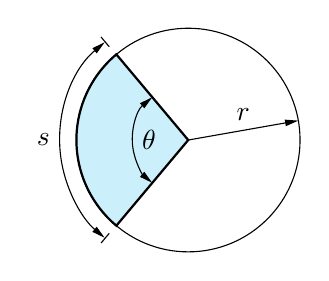
\begin{tikzpicture}[scale=0.71,>={[inset=0,angle'=27]Stealth}]
          \draw circle(2);
          \draw [thick,fill=cyan!20](230:2)--(0,0)--(130:2) arc (130:230:2)--cycle;
          \draw [->] (0, 0) -- node[above]{$r$} (10:2);
          \draw [|<->|](130:2.3) arc (130:230:2.3) node[left,pos=.5]{$s$};
          \draw [<->]  (130:1)   arc (130:230:1)   node[right,pos=.5]{$\theta$};
        \end{tikzpicture}
       \end{tabularx}
      \end{figure}

     \vspace{-0.5em}
    \item 

      直角三角形: 畢氏定理 (Pythagorean Theorem) $c^2 = a^2 + b^2$ \\
      證明: 由直角三角形面積公式 $\ds\frac{1}{2}\,c\cdot\overline{CO} = \frac{1}{2}\,a\cdot b\ie\overline{CO} = \frac{ab}{c}$. 又 $\ds\Delta ABC\sim\Delta CBO\sim\Delta ACO$, 則 $\ds\overline{AC}:\overline{BC} = \overline{CO}:\overline{BO} = \overline{AO}:\overline{CO}\ie b:a = \frac{ab}{c}: \overline{BO} = \overline{AO}: \frac{ab}{c} \ie \overline{BO} = \frac{a^2}{c},\,\overline{AO} = \frac{b^2}{c}$. 由 $\ds\overline{AB} = \overline{AO} + \overline{BO}\ie c = \frac{b^2}{c} + \frac{a^2}{c}\ie c^2 = a^2 + b^2$. 
      \vspace{-1em}
      \begin{figure}[!htbp]
        \centering
        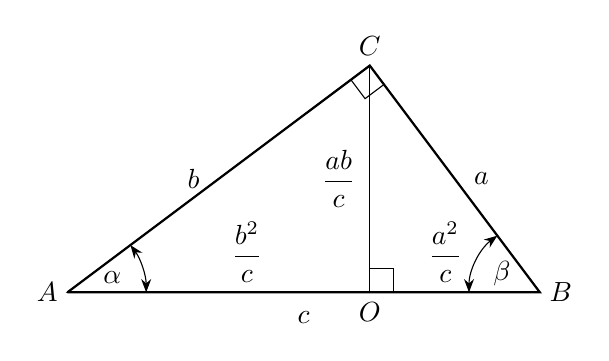
\begin{tikzpicture}[scale=1.2, >={Stealth[scale=1]}]
          \draw (0, 0) node[left] {$A$};
          \draw (16 / 5, 0) node[below] {$O$};
          \draw (5, 0) node[right] {$B$};
          \draw (16 / 5, 12 / 5) node[above] {$C$};
          \draw (41 / 10 + 0.1, 6 / 5) node[right] {$a$};
          \draw (8 / 5 - 0.1, 6 / 5) node[left] {$b$};
          \draw (2.5, -0.1) node[below] {$c$};
          \draw (16 / 5 - 0.05, 6 / 5) node[left] {$\ds\frac{ab}{c}$};
          \draw (8 / 5 + 0.3, 0) node[above] {$\ds\frac{b^2}{c}$};
          \draw (16 / 5 + 8 / 10, 0) node[above] {$\ds\frac{a^2}{c}$};
          \draw[thick] (0, 0) -- (5, 0) -- (16 / 5, 12 / 5) -- (0, 0);
          \draw (16 / 5, 0) -- (16 / 5, 12 / 5);
          \draw (5, 0) coordinate (a) -- (16 / 5, 0) coordinate (b) -- (16 / 5, 12 / 5) coordinate (c) pic [draw,angle radius=3mm] {right angle = a--b--c};
          \draw (5, 0) coordinate (a) -- (16 / 5, 12 / 5) coordinate (b) -- (0, 0) coordinate (c) pic [draw,angle radius=3mm] {right angle = a--b--c};
          \draw (16 / 5, 0) coordinate (a) -- (0, 0) coordinate (b) -- (16 / 5, 12 / 5) coordinate (c) pic ["$\alpha$",draw,<->,angle radius=10mm] {angle = a--b--c};
          \draw (16 / 5, 12 / 5) coordinate (a) -- (5, 0) coordinate (b) -- (16 / 5, 0) coordinate (c) pic ["$\beta$",draw,<->,angle radius=9mm] {angle = a--b--c};
        \end{tikzpicture}
      \end{figure}
      %\newpage
    \item 銳角三角函數
      \begin{figure}[!htbp]
        \centering
        \begin{tabularx}{0.7\textwidth}{X>{\centering\arraybackslash}X}
          \begin{align*}
            \sin\alpha = \frac{a}{c}\qquad\csc\alpha = \frac{c}{a} \\
            \cos\alpha = \frac{b}{c}\qquad\sec\alpha = \frac{c}{b} \\
            \tan\alpha = \frac{a}{b}\qquad\cot\alpha = \frac{b}{a} 
          \end{align*}
        &  
        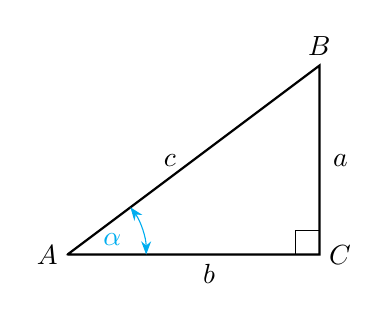
\begin{tikzpicture}[scale=1,>={Stealth[scale=1]}]
          \draw (0, 0) node[left] {$A$};
          \draw (16 / 5, 0) node[right] {$C$};
          \draw (16 / 5, 12 / 5) node[above] {$B$};
          \draw (8 / 5 - 0.1, 6 / 5) node[left] {$c$};
          \draw (16 / 5 + 0.05, 6 / 5) node[right] {$a$};
          \draw (8 / 5 + 0.2, 0) node[below] {$b$};
          \draw[thick] (0, 0) -- (16 / 5, 0) -- (16 / 5, 12 / 5) -- (0, 0);
          \draw (0, 0) coordinate (a) -- (16 / 5, 0) coordinate (b) -- (16 / 5, 12 / 5) coordinate (c) pic [draw,angle radius=3mm] {right angle = a--b--c};
          \draw (16 / 5, 0) coordinate (a) -- (0, 0) coordinate (b) -- (16 / 5, 12 / 5) coordinate (c) pic ["$\alpha$",draw,<->,cyan,angle radius=10mm] {angle = a--b--c};
        \end{tikzpicture}
       \end{tabularx}
      \end{figure}
    \item 廣義角三角函數
      \begin{figure}[!htbp]
        \centering
        \begin{tabularx}{0.7\textwidth}{X>{\centering\arraybackslash}X}
          \begin{align*}
            \sin\alpha = \frac{y}{r}\qquad\csc\alpha = \frac{r}{y} \\
            \cos\alpha = \frac{x}{r}\qquad\sec\alpha = \frac{r}{x} \\
            \tan\alpha = \frac{y}{x}\qquad\cot\alpha = \frac{x}{y} 
          \end{align*}
        &  
        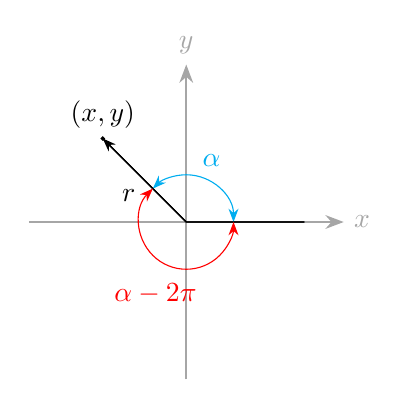
\begin{tikzpicture}[scale=1.,>={Stealth[scale=1]}]
          \draw[thick,gray!70,->] (-2, 0) -- (2, 0) node[right] {$x$};
          \draw[thick,gray!70,->] (0, -2) -- (0, 2) node[above] {$y$};
          \draw[->] (0, 0) -- (-1.06, 1.06);
          \filldraw (-1.06, 1.06) circle[radius=0.6pt];
          \draw (3 / 2, 0) coordinate (a) -- (0, 0) coordinate (b) -- (-1.06, 1.06) coordinate (c) pic ["$\alpha$", draw,<->,cyan,angle radius=6mm,angle eccentricity=1.4] {angle = a--b--c};
          \draw (-1.06, 1.06) coordinate (a) -- (0, 0) coordinate (b) -- (3 / 2, 0) coordinate (c) pic ["$\alpha - 2\pi$", draw,<->,red,angle radius=6mm,angle eccentricity=1.4,pic text options={shift={(-2pt,-4pt)}}] {angle = a--b--c};
          \draw (-1.06, 1.06) node[above] {$(x, y)$};
          \draw (-0.53 - 0.2, 0.53) node[below] {$r$};
        \end{tikzpicture}
       \end{tabularx}
      \end{figure}
  \end{itemize}
\end{dfn}

\begin{prp} 常用規則
  \setlength{\columnsep}{-30mm}
  \begin{multicols}{2}
    \begin{itemize}\setlength\itemsep{0em}
      \item $\sin(-\alpha) = -\sin\alpha$, $\cos(-\alpha) = \cos\alpha$. 
      \item $\forall\,n\in\mathbb{Z}$:  $\sin n\pi = 0$, $\cos n\pi = (-1)^n$. 
      \item $\sin^2\alpha + \cos^2\alpha = 1$, $\tan^2\alpha + 1 = \sec^2\alpha$, $\cot^2\alpha + 1 = \csc^2\alpha$. 
    \end{itemize}
  \end{multicols}
\end{prp}

\begin{prp} 和角公式 (addition formula)  
  \setlength{\columnsep}{-0mm}
  \begin{multicols}{2}
    \begin{itemize}\setlength\itemsep{0em}
      \item $\sin(\alpha\pm\beta) = \sin\alpha\cos\beta\pm\cos\alpha\sin\beta$
      \item $\cos(\alpha\pm\beta) = \cos\alpha\cos\beta\mp\sin\alpha\sin\beta$
    \end{itemize}
  \end{multicols}
\end{prp}

\begin{prp} 兩倍角公式 
  \setlength{\columnsep}{-0mm}
  \begin{multicols}{2}
    \begin{itemize}\setlength\itemsep{0em}
      \item $\ds\sin 2\alpha = 2\sin\alpha\cos\alpha$
      \item $\ds\cos 2\alpha = \cos^2\alpha - \sin^2\alpha$
      \item $\ds\cos^2 x = \frac{1 + \cos 2x}{2}$, $\ds\sin^2 x = \frac{1 - \cos 2x}{2}$
    \end{itemize}
  \end{multicols}
\end{prp}

\begin{prp} 積化和差公式 
  \setlength{\columnsep}{-0mm}
  \begin{multicols}{2}
    \begin{itemize}\setlength\itemsep{0em}
      \item $\ds\sin\alpha\cos\beta = \frac{1}{2}\,\big(\sin(\alpha - \beta) + \sin(\alpha + \beta)\big)$
      \item $\ds\cos\alpha\cos\beta = \frac{1}{2}\,\big(\cos(\alpha - \beta) + \cos(\alpha + \beta)\big)$
      \item $\ds\sin\alpha\sin\beta = \frac{1}{2}\,\big(\cos(\alpha - \beta) - \cos(\alpha + \beta)\big)$
    \end{itemize}
  \end{multicols}
\end{prp}

\begin{prf}[和角公式]
  設 $p = (1, 0)$, $q = (\cos(\alpha+\beta), \sin(\alpha+\beta))$. 座標系旋轉 $\alpha$ 後, $p = (\cos\alpha, -\sin\alpha)$, $q = (\cos\beta, \sin\beta)$. $p$, $q$ 距離不變 $\ie$ $\ds\sqrt{(\cos(\alpha+\beta) - 1)^2 + \sin^2(\alpha + \beta)} = \sqrt{(\cos\beta - \cos\alpha)^2 + (\sin\beta + \sin\alpha)^2}$ $\ie$ $\cos(\alpha + \beta) = \cos\alpha\cos\beta-\sin\alpha\sin\beta$. 代入 $\ds\alpha = x$, $\ds\beta = -\frac{\pi}{2}$ 可得 $\ds\sin x = \cos\big(x - \frac{\pi}{2}\big)$, 則 $\ds\sin(\alpha + \beta) = \cos\big(\alpha + \beta - \frac{\pi}{2}\big) = \cos\alpha \cos\big(\beta - \frac{\pi}{2}\big) - \sin\alpha\sin\big(\beta - \frac{\pi}{2}\big) = \cos\alpha\sin\beta - \sin\alpha\cos\big(\beta - \pi\big) = \cos\alpha\sin\beta - \sin\alpha(\cos\beta\cos\pi + \sin\beta\sin\pi) = \cos\alpha\sin\beta + \sin\alpha\cos\beta$.  
\end{prf}

\begin{figure}[!htbp]
  \centering
  \begin{tikzpicture}[scale=3, >={Stealth[scale=1]}]
    \draw[thick,gray!70,->] (0, 0) -- (1.5, 0) node[right] {$x$};
    \draw[thick,gray!70,->] (0, 0) -- (0, 1.2) node[above] {$y$};
    \draw (0, 0) -- (0.866, 0.5);
    \draw (0, 0) -- (-0.866, 0.5);
    \filldraw (1, 0) circle[radius=0.6pt];
    \filldraw (-0.866, 0.5) circle[radius=0.6pt];
    %\filldraw (0.866, 0.5) circle[radius=0.6pt];
    \draw (1, 0) coordinate (a) -- (0, 0) coordinate (b) -- (0.866, 0.5) coordinate (c) pic ["$\alpha$", draw,<->,red,angle radius=10mm] {angle = a--b--c};
    \draw (0.866, 0.5) coordinate (a) -- (0, 0) coordinate (b) -- (-0.866, 0.5) coordinate (c) pic ["$\beta$", draw,<->,blue,angle radius=10mm] {angle = a--b--c};
    \draw (1, 0) node[below] {$p$};
    \draw (-0.866, 0.5) node[above] {$q$};
    \draw (1 / 2, 0) node[below] {$\ds 1$};
    \draw (-0.866 / 2, 0.5 / 2) node[below] {$\ds 1$};
  \end{tikzpicture}
  \hspace{2cm}
  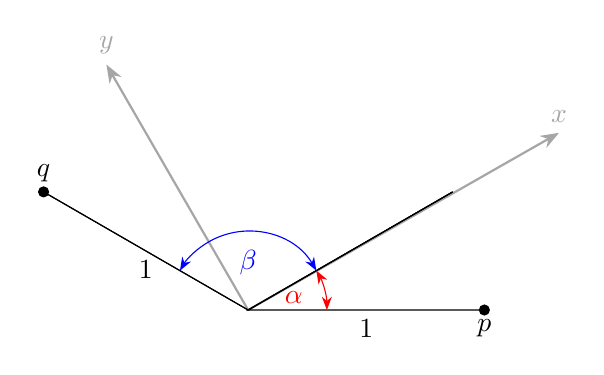
\begin{tikzpicture}[scale=3, >={Stealth[scale=1]}]
    \draw[thick,gray!70,->] (0, 0) -- (1.316, 0.75) node[above] {$x$};
    \draw[thick,gray!70,->] (0, 0) -- (-0.6, 1.0392) node[above] {$y$};
    \draw (0, 0) -- (0.866, 0.5);
    \draw (0, 0) -- (-0.866, 0.5);
    %\filldraw (0.866, 0.5) circle[radius=0.6pt];
    \filldraw (1, 0) circle[radius=0.6pt];
    \filldraw (-0.866, 0.5) circle[radius=0.6pt];
    \draw (1, 0) coordinate (a) -- (0, 0) coordinate (b) -- (0.866, 0.5) coordinate (c) pic ["$\alpha$", draw,<->,red,angle radius=10mm] {angle = a--b--c};
    \draw (0.866, 0.5) coordinate (a) -- (0, 0) coordinate (b) -- (-0.866, 0.5) coordinate (c) pic ["$\beta$", draw,<->,blue,angle radius=10mm] {angle = a--b--c};
    \draw (1, 0) node[below] {$p$};
    \draw (-0.866, 0.5) node[above] {$q$};
    \draw (1 / 2, 0) node[below] {$\ds 1$};
    \draw (-0.866 / 2, 0.5 / 2) node[below] {$\ds 1$};
  \end{tikzpicture}
\end{figure}

\section*{0.11 反三角函數}

\begin{dfn}
  在以下定義域上之三角函數為嵌射: 
  \begin{align*}
    &\sin x: \big[-\frac{\pi}{2}, \frac{\pi}{2}\big]\to[-1, 1] &\csc x: \big(0, \frac{\pi}{2}\big]\cup\big(\pi, \frac{3\pi}{2}\big]\to(-\infty, -1]\cup[1,\infty) \\
    &\cos x: \big[0, \pi\big]\to[-1, 1] &\sec x: \big[0, \frac{\pi}{2}\big)\cup\big[\pi, \frac{3\pi}{2}\big)\to(-\infty, -1]\cup[1,\infty) \\
    &\tan x: \big(-\frac{\pi}{2}, \frac{\pi}{2}\big)\to(-\infty, \infty) &\cot x: \big(0, \pi\big)\to(-\infty, \infty)\qquad\qquad
  \end{align*}
  故存在反三角函數: 
  \begin{align*}
   &\sin^{-1} x: [-1, 1]\to\big[-\frac{\pi}{2}, \frac{\pi}{2}\big] &\csc^{-1} x: (-\infty, -1]\cup[1,\infty)\to\big(0, \frac{\pi}{2}\big]\cup\big(\pi, \frac{3\pi}{2}\big] \\
   &\cos^{-1} x: [-1, 1]\to\big[0, \pi\big] &\sec^{-1} x: (-\infty, -1]\cup[1,\infty)\to\big[0, \frac{\pi}{2}\big)\cup\big[\pi, \frac{3\pi}{2}\big) \\
   &\tan^{-1} x: (-\infty, \infty)\to\big(-\frac{\pi}{2}, \frac{\pi}{2}\big) &\cot x: (-\infty, \infty)\to\big(0, \pi\big)\qquad\qquad
 \end{align*}
\end{dfn}

\vspace{-1cm}
\begin{figure}[!htbp]
  \centering
  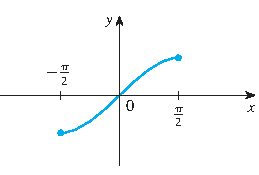
\includegraphics[height=.25\textheight,page=1]{fig/trig.pdf}\hspace{2cm}
  \includegraphics[height=.25\textheight,page=2]{fig/trig.pdf}
  \caption{$y = \sin x$, $y = \sin^{-1} x$}
\end{figure}

\vspace{-1cm}
\begin{figure}[!htbp]
  \centering
  \includegraphics[height=.25\textheight,page=3]{fig/trig.pdf}\hspace{2cm}
  \includegraphics[height=.25\textheight,page=4]{fig/trig.pdf}
  \caption{$y = \cos x$, $y = \cos^{-1} x$}
\end{figure}

\vspace{-1cm}
\begin{figure}[!htbp]
  \centering
  \includegraphics[height=.25\textheight,page=5]{fig/trig.pdf}\hspace{2cm}
  \includegraphics[height=.25\textheight,page=6]{fig/trig.pdf}
  \caption{$y = \tan x$, $y = \tan^{-1} x$}
\end{figure}

\begin{prp}
  \begin{itemize}\setlength\itemsep{0em}
    \item[]
    \item 當 $\ds-\frac{\pi}{2}\leqslant x\leqslant\frac{\pi}{2}$, $\sin^{-1}(\sin x) = x$, $\tan^{-1}(\tan x) = x$; 當 $\ds 0\leqslant x\leqslant\pi$, $\cos^{-1}(\cos x) = x$.  
    \item 當 $\ds-1\leqslant x\leqslant1$, $\sin(\sin^{-1} x) = x$, $\cos(\cos^{-1} x) = x$; 當 $\ds-\infty < x < \infty$, $\tan(\tan^{-1} x) = x$. 
    \item $\sin^{-1}(-x) = -\sin^{-1}x$; $\tan^{-1}(-x) = -\tan^{-1}x$; $\cos^{-1}(-x) = \pi - \cos^{-1}x$. 
  \end{itemize}
\end{prp}

\begin{ex} 基本反三角函數求值. 
  \setlength{\columnsep}{-5mm}
  \begin{multicols}{4}
  \begin{enumerate}
    \item $\ds\sin^{-1}\frac{\sqrt{3}}{2} = \frac{\pi}{3}$
    \item $\ds\cos^{-1}\Big(-\frac{1}{2}\Big) = \frac{2\pi}{3}$%\quad\text{ ($[0,\,\pi]$ 對稱) }$
    \item $\ds\tan^{-1}1 = \frac{\pi}{4}$ 
    \item $\ds\cos\Big(\sin^{-1}\frac{3}{5}\Big) = \frac{4}{5}$
  \end{enumerate}
\end{multicols}
\end{ex}

\begin{ex}
  若 $\ds\alpha = \sin^{-1}\frac{2}{3}$, 求 $\cos\alpha$, $\tan\alpha$, $\cot\alpha$, $\sec\alpha$, $\csc\alpha$. 
\end{ex}

\begin{sol}
  $\ds\cos\alpha = \frac{\sqrt{5}}{3}$, $\ds\tan\alpha = \frac{2}{\sqrt{5}}$, $\ds\cot\alpha = \frac{\sqrt{5}}{2}$, $\ds\sec\alpha = \frac{3}{\sqrt{5}}$, $\ds\csc\alpha = \frac{3}{2}$. 
\end{sol}

\begin{ex}
  若 $\ds f(x) = \frac{1}{\sin^{-1}\big(\frac{1}{x}\big)}$, 求 $\dom{f}$. 
\end{ex}

\begin{sol}
  $\dom f = \big\{x\,|\, -1\leqslant\frac{1}{x}\leqslant 1\big\} = (-\infty,-1]\,\cup\,[1,\infty)$. 
\end{sol}

\begin{ex}
  令 $\ds f(x) = \sin(\sin^{-1} x)$, $\ds g(x) = \sin^{-1}(\sin x)$, 求 $\dom{f}$, $\dom{g}$ 與其圖形. 
\end{ex}

\begin{sol}
  \begin{itemize}\setlength\itemsep{0em}
    \item[]
    \item $\dom f = \dom{\sin^{-1}} = [-1, 1]$; $f(x) = x$, $\forall\,x\in[-1, 1]$. 
    \item $\ds\dom g = \mathbb{R}$; $\ds g(x) = \begin{cases} -x + (2n + 1)\,\pi & x\in[(2n + \frac{1}{2})\,\pi,\, (2n + \frac{3}{2})\,\pi) \\ x - (2n + 2)\,\pi & x\in[(2n + \frac{3}{2})\,\pi,\, (2n + \frac{5}{2})\,\pi)\end{cases}\quad n\in\mathbb{Z}$. 
    %\vspace{-1cm}
    \begin{figure}[!htbp]
      \centering
      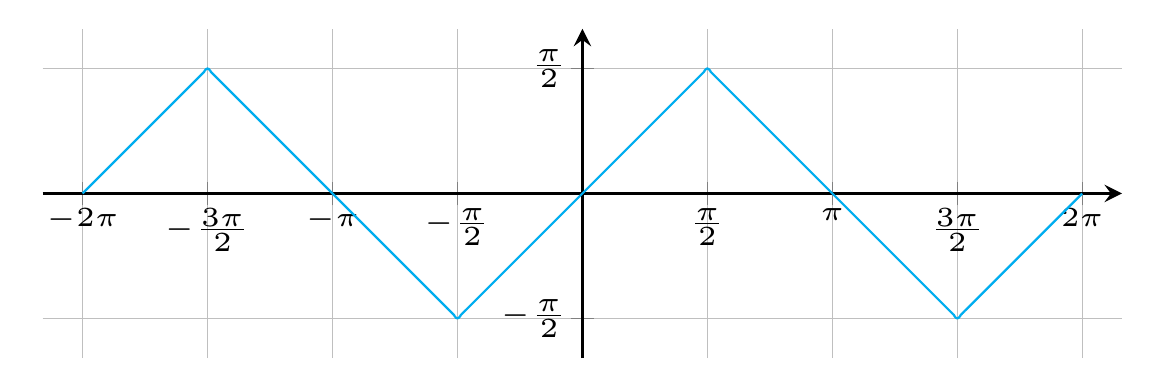
\begin{tikzpicture}[scale=2.]
        \begin{axis}%
          [grid=both,
           unit vector ratio*=1 1 1,
           minor tick num=1,
           grid style={line width=.1pt, draw=gray!10},
           major grid style={line width=.2pt,draw=gray!50},
           axis lines=middle,
           xtick={-6.28318, -4.7123889, -3.14159, -1.5708, 1.5708, 3.14159, 4.7123889, 6.28318},
           xticklabels={$-2\pi$, $-\frac{3\pi}{2}$, $-\pi$, $-\frac{\pi}{2}$, $\frac{\pi}{2}$, $\pi$, $\frac{3\pi}{2}$, $2\pi$},
           ytick={-1.5708, 1.5708},
           yticklabels={$-\frac{\pi}{2}$, $\frac{\pi}{2}$},
           x tick label style={yshift=0.3em},
           y tick label style={xshift=0.3em},
           enlargelimits={abs=0.5}
          ]
          \addplot[domain=-2*pi:2*pi,samples=3000,smooth,cyan] {rad(asin(sin(deg(x))))};
        \end{axis}
      \end{tikzpicture}
      \caption{$g(x) = \sin^{-1}(\sin x)$}
    \end{figure}
  \end{itemize}
\end{sol}

\begin{ex}
  將 $\ds\sin(\cos^{-1} x)$ 與 $\tan(\cos^{-1} x)$ 化簡為 $x$ 的 (不含三角函數之) 表示式, 其中 $-1\leqslant x\leqslant 1$. 
\end{ex}

\begin{sol}
  令 $\ds u =\cos^{-1}x$, 則 $\ds0\leqslant u\leqslant\pi$, $\cos u = x$, $\ds\sin u = +\sqrt{1 - x^2}$, $\ds\tan u = \frac{\sqrt{1 - x^2}}{x}$. 
\end{sol}

\begin{ex} 化簡以下表示式. 
  \setlength{\columnsep}{-0mm}
  \begin{multicols}{3}
    \begin{enumerate}\setlength\itemsep{0em}
      \item $\cos(\sin^{-1} x)$
      \item $\sin(\tan^{-1} x)$
      \item $\sin(2\tan^{-1} x)$
    \end{enumerate}
  \end{multicols}
\end{ex}

\begin{sol} 
  \setlength{\columnsep}{-0mm}
  \begin{multicols}{3}
  \begin{enumerate}\setlength\itemsep{0em}
    \item $\ds\cos(\sin^{-1} x) = \sqrt{1 - x^2}$
    \item $\ds\sin(\tan^{-1} x) = \frac{x}{\sqrt{1 + x^2}}$
    \item $\ds\sin(2\tan^{-1} x) = \frac{2x}{1 + x^2}$
  \end{enumerate}
  \end{multicols}
\end{sol}

\begin{ex}
  將 $\ds \sin(\cos^{-1} x + \tan^{-1}y)$ 化簡為 $x$, $y$ 的 (不含三角函數之) 表示式, 其中 $-1\leqslant x\leqslant 1$, $y\in\mathbb{R}$. 
\end{ex}

\begin{sol}
  令 $\ds u =\cos^{-1}x$, $\ds v=\tan^{-1} y$, 則 $\cos u = x$, $\tan v = y$, 由此 $\ds\sin u = \sqrt{1 - x^2}$, $\ds\cos v = \frac{1}{\sqrt{1 + y^2}}$, $\ds\sin v = \frac{y}{\sqrt{1 + y^2}}$; 原式為 $\ds\sin(\cos^{-1} x + \tan^{-1}y) = \sin(u + v) = \sin u\cos v + \cos u\sin v = \sqrt{1 - x^2}\cdot\frac{1}{\sqrt{1 + y^2}} + x\cdot\frac{y}{\sqrt{1 + y^2}}$. 
\end{sol}

\begin{ex}
  證明 $\ds\cos^{-1}(1 - 2x^2) = 2\sin^{-1}x$, $0\leqslant x\leqslant 1$. 
\end{ex}

\begin{sol}
  令 $\ds u = \sin^{-1}x$, 則 $\ds\cos^{-1}(1 - 2x^2) = \cos^{-1}(1 - 2\sin^2u) = \cos^{-1}(\cos 2u) = 2u = 2\sin^{-1}x$. 
\end{sol}

\begin{ex}
  解 $\ds2\sin^{-1} x + \cos^{-1}x = \pi$. 
\end{ex}

\begin{sol}
  令 $\ds\sin^{-1}x = u$, $\ds\cos^{-1}x = v$, 則 $\ds\sin u = \cos v = x$, $\ds\cos u = \sin v = \sqrt{1 - x^2}$. 方程式兩邊取 $\cos$ $\ds\ie\cos(2u + v) = -1 \ie \cos2u\cos v - \sin2u\sin v = (1 - 2\sin^2u)\cos v - 2\sin u\cos u\sin v = -1 \ie (1 - 2x^2)x - 2 x(1 - x^2) = -1 \ie x = 1$. 
\end{sol}

\myline

%\bibliographystyle{elsarticle-harv}
%\bibliography{note00}

\end{document}
